\documentclass[preprint,11pt]{elsarticle}

\usepackage{amsmath,amssymb}
\usepackage{booktabs}
\usepackage{graphicx}
\usepackage{hyperref}
\usepackage{xcolor}
\usepackage{siunitx}
\usepackage{seqsplit}

\graphicspath{{figures/}}
\hypersetup{hidelinks}

\journal{Infrared Physics \& Technology}
\biboptions{numbers,sort&compress}

\begin{document}
\sloppy

\begin{frontmatter}

\title{Confidence-Shielded Evaluator-Conditioned Fusion for Risk-Controlled Infrared--Visible Object Detection}

\author[AUTHOR]{Jianyong Zhao}
\ead{shaohaojia2001@163.com}
\ead[url]{https://orcid.org/0009-0005-3251-2785}

\author[AUTHOR]{Zigao Wu\corref{cor1}}
\ead{zgwu@ncepu.edu.cn}
\ead[url]{https://orcid.org/0000-0002-7449-343X}

\author[AUTHOR]{Mengfei Ma}
\ead{MYmmf01@163.com}
\ead[url]{https://orcid.org/0009-0007-1328-1314}

\cortext[cor1]{Corresponding author.}
\affiliation[AUTHOR]{organization={North China Electric Power University},
            addressline={Hebei},
            city={Baoding},
            postcode={071003},
            country={China}}

\begin{abstract}
Infrared--visible image fusion is commonly treated as a preprocessing step
whose output should benefit any downstream detector. In practice, the same
fused image may improve one detector, leave another unchanged, and degrade a
third because detection utility depends on the learned detector representation
and confidence calibration. We introduce Confidence-Shielded
Evaluator-Conditioned Fusion (CS-ECF), a label-free input-arbitration policy
that evaluates visible, CDF, PIAFusion, and SPGFusion candidates with the target
detector itself. CS-ECF averages each candidate's five highest detection
confidences and permits a fused input only when its confidence exceeds that of
the visible image by a factor of 1.5; otherwise, it falls back to the visible
image. The margin was fixed on validation data before confirmatory testing. We
evaluated the frozen policy on LLVIP, a grouped six-class M3FD test set, and
three consecutive groups from the official DroneVehicle test split, comprising
12 detector checkpoints. Nine checkpoints improved, the dataset-balanced AP50
gain was 0.0133, and the model-by-group hierarchical 95\% interval was
[0.0028, 0.0213]. Removing the shield introduced a worst AP50 loss of 0.0584,
whereas the frozen policy limited the worst loss to 0.0040. The two
DroneVehicle checkpoints improved by 0.0251 and 0.0293, although they belong to
the same training run. M3FD gains were concentrated in the people class, and
LLVIP intervals crossed zero. These results support CS-ECF as a risk-controlled
evaluator-aware fusion-input system for pedestrian-centric and mixed
infrared--visible detection; they do not support uniform improvement across all
object classes. Under a standardized serial benchmark, candidate generation and
four detector evaluations required approximately \SI{0.71}{s} per image pair,
dominated by SPGFusion.
\end{abstract}

\begin{keyword}
infrared--visible image fusion \sep object detection \sep
evaluator-conditioned fusion \sep confidence calibration \sep
risk control \sep thermal imaging
\end{keyword}

\end{frontmatter}

\section{Introduction}

Infrared--visible imaging combines the spatial detail and color of visible
sensors with thermal evidence that can remain available when illumination is
poor, smoke reduces contrast, or targets have weak visual texture. This
complementarity has motivated pixel-, feature-, and network-based fusion methods
for surveillance, autonomous perception, and thermal imaging systems.
\cite{mudavath2026review,zhang2020,tang2022,zhang2026}
In detection-oriented applications, the value of a fused image is not determined
by visual appeal alone; it is the change in detector outputs under a specified
operating condition.

Current practice often selects one fused representation and evaluates it with
one detector on one benchmark. This design assumes that a globally preferred
fusion result remains preferable across detector architectures and training
seeds. The assumption is fragile because detectors differ in receptive fields,
confidence calibration, training data, and sensitivity to high-frequency
detail. Consequently, a fusion rule that improves one evaluator may reduce the
average precision (AP) of another on the same image.

Per-image selection offers a natural response: run several fusion candidates
and choose the one with the strongest detector response. Yet unconstrained
selection converts small calibration differences into frequent input switches
and can produce severe losses when a spurious high-confidence response is
mistaken for improved detection. The problem is therefore not only to predict
which fused image looks best, but to decide when the evidence is strong enough
to depart from the visible-image safety baseline.

Recent infrared--visible fusion and detection studies have optimized shared
fusion networks, cross-modal feature fusion, or hierarchical detectors
\cite{zhao2025cmifdf,gao2026coifsd,an2026mrtdetr,zhang2026hffn}. These studies
establish the relevance of joint fusion and detection, but they generally train
or optimize a detector-fusion system. They do not establish a label-free
arbitration rule whose switching threshold is fixed independently of the
confirmatory tests and whose behavior is reported at the level of detector
checkpoint, image, and scene or frame group.

We formulate infrared--visible fusion selection as evaluator-conditioned input
arbitration. CS-ECF evaluates four candidates with the target detector, computes
a top-five confidence score, and accepts a fused candidate only when its score
reaches 1.5 times that of the visible input. The threshold is selected on
validation data and frozen before testing. We evaluate the policy on LLVIP,
M3FD, and DroneVehicle with model-, image-, and group-aware uncertainty,
compare it with fixed fusion and an unshielded selector, and report the cost and
failure boundaries. The contributions are:
\begin{enumerate}
  \item an evaluator-conditioned formulation of fusion-input selection that does
  not use test labels;
  \item a confidence shield that reduces catastrophic switching while retaining
  positive dataset-balanced gains;
  \item a three-dataset confirmation that separates image-level uncertainty,
  scene/group uncertainty, and checkpoint variability, including explicit
  evidence that the M3FD gain is concentrated in the people class.
\end{enumerate}

\section{Methods}

\subsection{Problem formulation}

Let \(x_v\) and \(x_i\) denote a registered visible--infrared pair, and let
\(\mathcal{D}\) denote the target detector checkpoint. A candidate
\(c\in\mathcal{C}\) produces an input image \(x_c\), where
\(\mathcal{C}=\{\mathrm{vis},\mathrm{cdf},\mathrm{pia},\mathrm{spg}\}\).
The policy returns one candidate per pair without access to ground-truth boxes:
\begin{equation}
g(x_v,x_i;\mathcal{D})\in\mathcal{C}.
\end{equation}
The final detection output is
\(\mathcal{D}(x_{g(x_v,x_i;\mathcal{D})})\). The detector is therefore reused
for candidate evaluation and final inference; it is not an external label
oracle.

\subsection{Fusion candidates}

The visible input is always included as a safety candidate. CDF combines a
pixel-mean image and an IFCNN image through sign-consistent high-frequency
details:
\begin{equation}
d(x)=
\begin{cases}
\operatorname{sign}(d_m+d_i)\min(|d_m|,|d_i|), & d_m d_i>0,\\
0, & \text{otherwise}.
\end{cases}
\end{equation}
A thermal-validity mask \(M\) is formed from the infrared top-hat response,
infrared intensity, visible luminance, connected components, and smoothing.
The shared detail is injected into the LAB luminance channel:
\begin{equation}
L' = L + \alpha M d.
\end{equation}
The frozen settings are \(q=0.95\), \(\alpha=0.20\), and \(\sigma=5\).
PIAFusion and SPGFusion are generated with their official model definitions and
pretrained weights under the same image-pair protocol.
\cite{zhang2020,tang2022,zhang2026}

\subsection{Confidence-shielded arbitration}

For candidate \(c\), let
\(s_{c,1}\ge s_{c,2}\ge\cdots\) be detector confidences. We define
\begin{equation}
q_c=\frac{1}{\min(K,n_c)}
\sum_{j=1}^{\min(K,n_c)}s_{c,j},
\qquad K=5,
\end{equation}
where \(n_c\) is the number of detections. Candidates with no detections receive
\(q_c=-1\). The highest-scoring candidate is
\(c^\ast=\arg\max_c q_c\), with ties resolved in favor of visible. The selected
input is
\begin{equation}
c=
\begin{cases}
c^\ast, & c^\ast\ne\mathrm{vis}\ \text{and}\ q_{c^\ast}\ge1.5q_{\mathrm{vis}},\\
\mathrm{vis}, & \text{otherwise}.
\end{cases}
\end{equation}
The margin \(1.5\) was selected on validation data before the confirmatory
tests. The selector uses no test labels and makes no class-specific decision.

\subsection{Datasets and evaluators}

LLVIP supplies a 300-image pedestrian test set spanning seven scenes
\cite{jia2021}. M3FD supplies a grouped six-class test set of 200 images
\cite{liu2022}, split by consecutive frame groups to reduce adjacent-frame
leakage; the detector families are YOLO26n and YOLOv8n. DroneVehicle contributes
300 image pairs from three fixed consecutive
100-frame groups of the official test archive. The groups were selected with a
predefined seed of 2037 before evaluation. The YOLO11x-OBB best and last
checkpoints were both evaluated. The source archive has 4,430,343,899 bytes and
SHA-256
\texttt{\seqsplit{94BF47E493E7A57FD5D900439F614F339E7B6C7181E4D781BCFEBAEB963FFD8E}}
\cite{sun2022}.
All OBB outputs use a confidence floor of 0.001 and an NMS IoU threshold of 0.7.

\begin{table}[t]
\centering
\small
\caption{Datasets and confirmatory evaluation units.}
\label{tab:data}
\begin{tabular}{@{}llrrl@{}}
\toprule
Dataset & Split & Images & Classes & Evaluation groups \\
\midrule
LLVIP & Official test & 300 & 1 & 7 scenes \\
M3FD & Grouped test & 200 & 6 & 2 frame groups \\
DroneVehicle & Official test subset & 300 & 1 OBB vehicle & 3 frame groups \\
\bottomrule
\end{tabular}
\end{table}

\subsection{Statistical analysis}

Point estimates use pooled AP50 after concatenating detections across test
images within a checkpoint. Image bootstrap intervals resample images within a
checkpoint. Group bootstrap intervals resample scenes or consecutive frame
groups and are the primary clustered intervals. The dataset-balanced estimand
assigns equal weight to LLVIP, M3FD, and DroneVehicle and resamples checkpoints
and groups. M3FD has only two test groups and LLVIP has seven scenes, so the
group bootstrap is reported as a finite-cluster analysis. The model-by-group
bootstrap used 500 resamples with \texttt{numpy.random.default\_rng(2219)} in
Python 3.10.22 and NumPy 2.2.6. Spearman association tests used SciPy 1.15.3.

\subsection{Implementation and cost}

At a standardized fusion input of \(384\times512\), FP32 and batch size one on
an NVIDIA RTX 2080 Ti, the CDF pipeline required \SI{22.3}{ms}, PIAFusion
\SI{37.7}{ms}, and SPGFusion \SI{516.3}{ms}. Four serial YOLO11x-OBB evaluations
at an input size of 640 required \SI{130.0}{ms}, giving an estimated serial
total of \SI{706.3}{ms}. This estimate excludes model loading or swapping, data
loading, and final detection post-processing. SPGFusion's additional peak
activation memory was \SI{1453.5}{MiB}; per-stage memory values must not be
summed as an end-to-end peak.

\section{Results}

\subsection{Fusion utility is evaluator-dependent}

Across the 12 confirmatory checkpoints, the same candidate library produced
both positive and negative gains (Fig.~\ref{fig:evaluator}). CS-ECF improved
nine checkpoints. Its dataset-balanced AP50 gain was 0.0133, with a
model-by-group hierarchical 95\% interval of [0.0028, 0.0213]. The unshielded
selector improved seven of 12 checkpoints, had a larger dataset-balanced mean of
0.0332, and produced a worst loss of 0.0584.

\begin{figure*}[t]
\centering
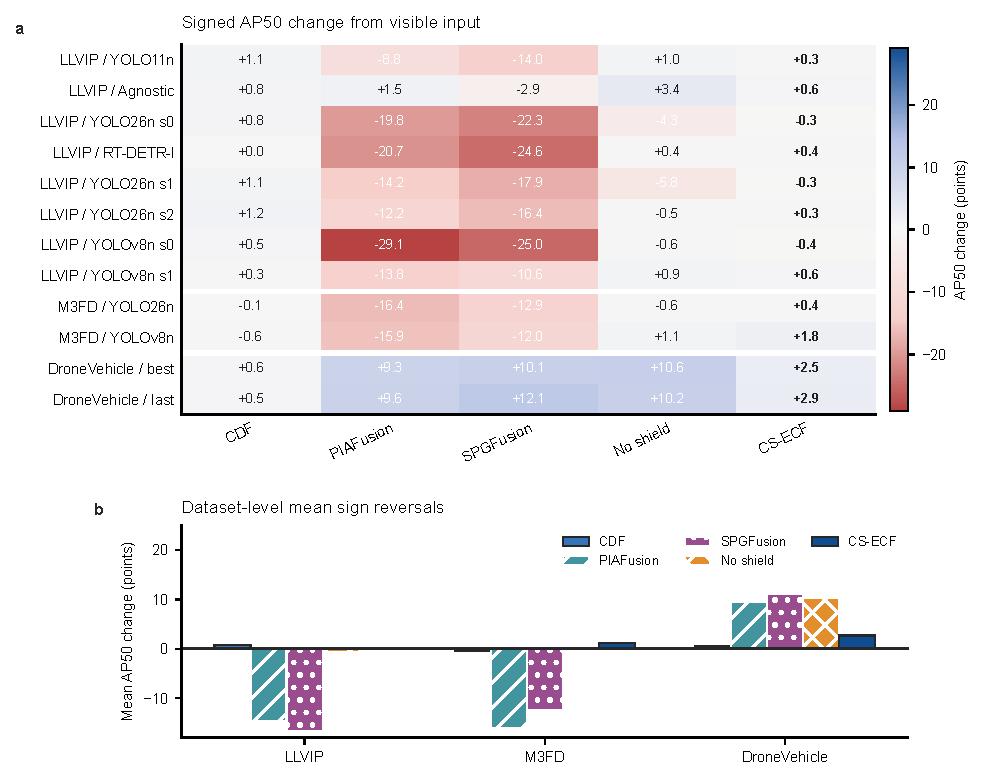
\includegraphics[width=\linewidth]{fig1_evaluator_dependence.pdf}
\caption{\textbf{Evaluator-dependent utility of infrared--visible fusion
candidates.} \textbf{a}, Signed AP50 change from the visible input for CDF,
PIAFusion, SPGFusion, the unshielded selector, and CS-ECF across 12 detector
checkpoints. Cells are point contrasts. \textbf{b}, Dataset-level mean AP50
changes. Equal candidate sets produce opposite signs across datasets. Source
data are provided in \texttt{figure1\_source.csv}.}
\label{fig:evaluator}
\end{figure*}

\subsection{Dataset-specific behavior}

On LLVIP, the mean gain was 0.0016 and five of eight checkpoints improved; the
model and image intervals crossed zero. On M3FD, both six-class checkpoints
improved, with a mean gain of 0.0111. On the independent DroneVehicle test
subset, the best and last OBB checkpoints improved by 0.0251 and 0.0293; the
combined group interval was [0.0002, 0.0406]. All three DroneVehicle groups were
non-negative, but one gained only 0.0002. The two OBB checkpoints originated
from the same training run and are not independent architectures.

\begin{table}[t]
\centering
\small
\caption{Confirmatory checkpoint summary and policy comparison.}
\label{tab:policy}
\begin{tabular}{@{}lrrrr@{}}
\toprule
Policy & Positive & Mean & Dataset-balanced & Worst \\
\midrule
Always CDF & 10/12 & +0.0052 & +0.0031 & -0.0059 \\
Always PIAFusion & 3/12 & -0.1087 & -0.0710 & -0.2910 \\
Always SPGFusion & 2/12 & -0.1136 & -0.0602 & -0.2501 \\
Top-5 no shield & 7/12 & +0.0132 & +0.0332 & -0.0584 \\
CS-ECF & 9/12 & +0.0074 & +0.0133 & -0.0040 \\
\bottomrule
\end{tabular}
\end{table}

\subsection{The shield is a risk-control mechanism}

Without the shield, the policy selected fused candidates on most LLVIP and
DroneVehicle images and occasionally produced large confidence gains that did
not translate into AP. The 1.5 margin reduced switches and lowered the worst
AP50 loss from 0.0584 to 0.0040. On DroneVehicle, however, the shield also
reduced the mean gain from 0.1040 to 0.0272. This trade-off is the central
quantitative meaning of risk control in this study.

\begin{figure*}[t]
\centering
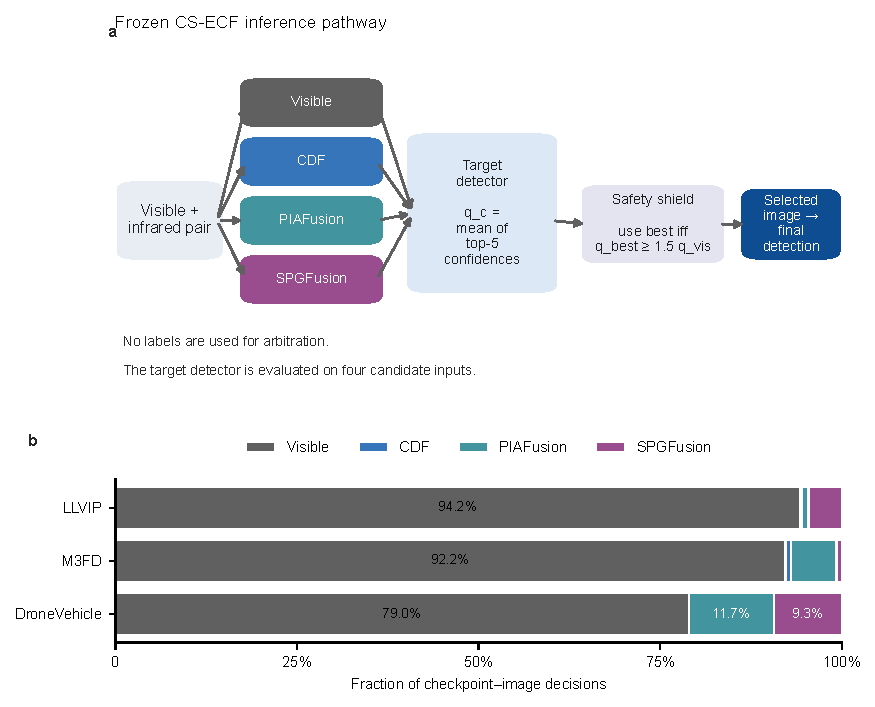
\includegraphics[width=\linewidth]{fig2_csecf_workflow.pdf}
\caption{\textbf{Confidence-shielded evaluator-conditioned fusion.}
\textbf{a}, The visible--infrared pair is passed to visible, CDF, PIAFusion,
and SPGFusion candidates. The target detector computes its top-five mean
confidence for each candidate. A fused candidate is selected only when its
score is at least 1.5 times the visible score; otherwise the visible input is
retained. No labels are used for arbitration. \textbf{b}, Composition of the
frozen decisions across all checkpoint--image trials. Source data are provided
in \texttt{figure2\_source.csv}.}
\label{fig:workflow}
\end{figure*}

\begin{figure*}[t]
\centering
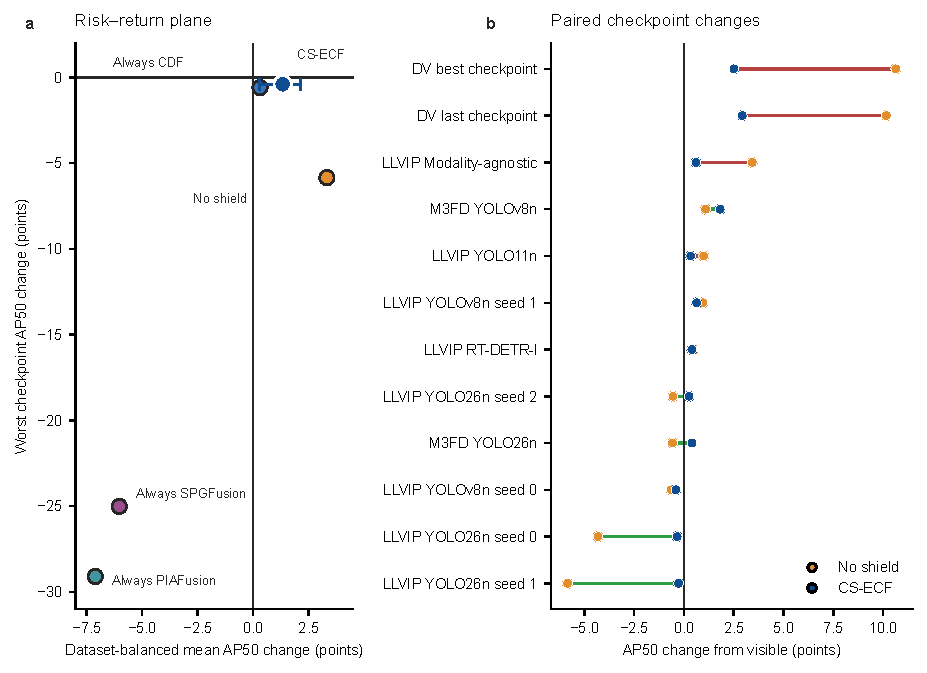
\includegraphics[width=\linewidth]{fig3_risk_return.pdf}
\caption{\textbf{Risk--return trade-off of fusion-input policies.}
\textbf{a}, Dataset-balanced mean AP50 change versus worst-checkpoint AP50
change. The CS-ECF horizontal error bar is the model-by-group hierarchical
95\% interval. \textbf{b}, Paired checkpoint changes under the unshielded
selector and CS-ECF. The shield sacrifices part of the DroneVehicle mean gain
to reduce the worst LLVIP loss. Source data are provided in
\texttt{figure3\_source.csv}.}
\label{fig:risk}
\end{figure*}

\subsection{Fixed baselines and class concentration}

Always CDF improved 10 of 12 checkpoints and had a dataset-balanced gain of
0.0031, but remained negative on both M3FD detectors. Always PIAFusion and
Always SPGFusion had negative dataset-balanced gains because their strong
DroneVehicle performance did not transfer to the other datasets. In the M3FD
six-class evaluation, the CS-ECF gain was concentrated in people:
YOLO26n improved by 0.0214 and YOLOv8n by 0.1090, while the other five classes
changed by at most 0.0003 in absolute AP50 (Fig.~\ref{fig:thermal}). The
evidence therefore supports a pedestrian/people-focused interpretation, not
uniform six-class improvement.

\subsection{Thermal feature association and mask ablation}

On LLVIP, infrared top-hat contrast showed a weak positive association with
switching (Spearman \(\rho=0.151\), \(p=0.009\)), whereas visible luminance was
only weakly negative (\(\rho=-0.104\), \(p=0.071\)). On M3FD, thermal contrast
showed a moderate positive association (\(\rho=0.320\), \(p<10^{-5}\)).
On DroneVehicle, however, both thermal contrast (\(\rho=-0.403\)) and visible
luminance (\(\rho=-0.441\)) were negatively associated with switching. A
high-thermal/low-visible median split did not produce a consistently larger AP
gain than the remaining images.

A fixed-input mask ablation gave a smaller but consistent thermal effect on
DroneVehicle. Replacing the thermal-validity mask with global detail injection
changed the CDF gain from 0.0060 to 0.0057 for the best checkpoint and from
0.0050 to 0.0038 for the last checkpoint. The thermal mask added 0.0007 AP50 on
average relative to global injection.

\begin{figure*}[t]
\centering
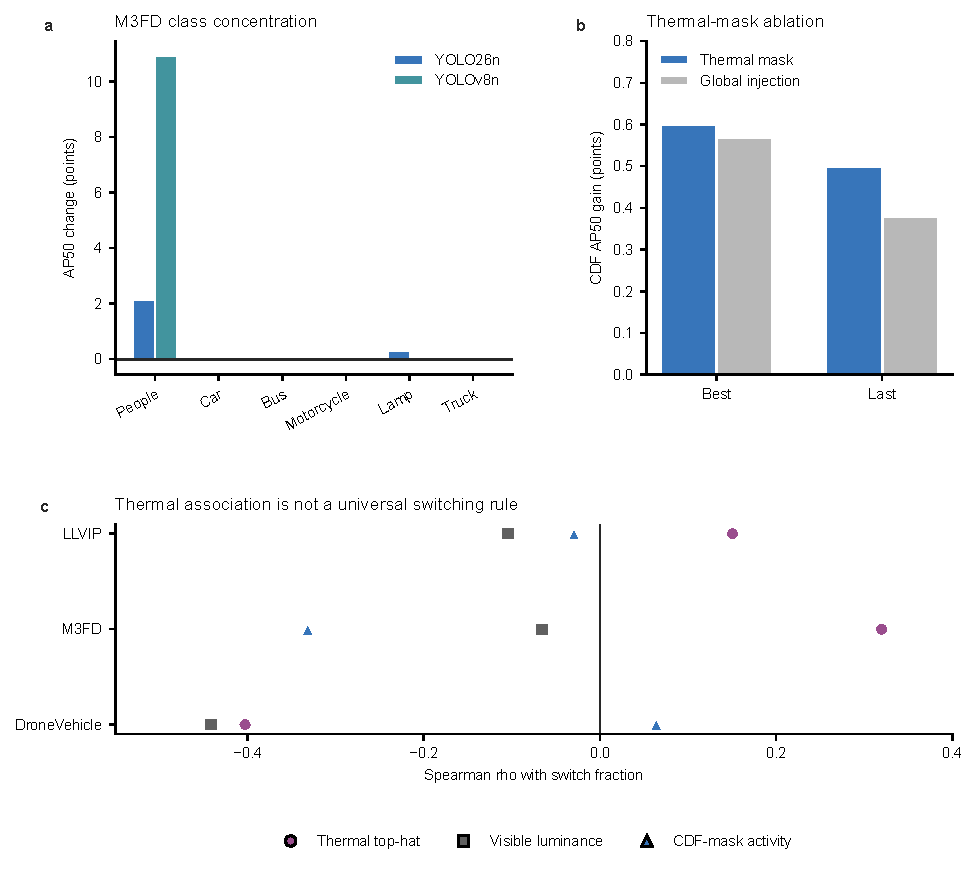
\includegraphics[width=\linewidth]{fig4_thermal_class_boundary.pdf}
\caption{\textbf{Thermal constraints and class-specific effects.}
\textbf{a}, M3FD AP50 changes for six classes. The gain is concentrated in
people. \textbf{b}, Fixed-input DroneVehicle CDF gain with the thermal-validity
mask or global detail injection. \textbf{c}, Spearman association between the
fused-selection fraction and thermal top-hat contrast, visible luminance, or
CDF-mask activity. The association reverses on DroneVehicle, which does not
support a universal thermal switching rule. Source data are provided in
\texttt{figure4\_source.csv}.}
\label{fig:thermal}
\end{figure*}

\clearpage
\section{Discussion}

The central finding is that fusion utility is not an intrinsic property of a
fused image alone. A candidate can improve one detector's confidence ordering
while harming another's, and a policy that ignores this dependence can select
inputs that appear confident but do not improve AP. CS-ECF responds by using
the target detector as an input arbiter and requiring a large visible-relative
margin before switching.

The shield's value is clearest in the tail. The unshielded selector achieved a
higher dataset-balanced average on DroneVehicle, where both PIAFusion and
SPGFusion were strong, but it also produced severe LLVIP losses. The 1.5 margin
deliberately favors visible fallback under ambiguous evidence. This is
consistent with a deployment rule in which a small probability of a large
regression is more costly than a missed opportunity for a moderate gain.

Two boundaries constrain the interpretation. First, the strongest M3FD effect
is class-specific: people detection improves substantially while the remaining
classes are nearly unchanged. The selected thermal evidence is therefore most
useful for a subset of target appearances, not all six vehicle classes. Second,
the DroneVehicle confirmation uses two checkpoints from the same training run.
The official test groups are independent of model selection, but the checkpoints
share training data and are correlated.

The thermal stratification adds another limitation. Thermal contrast may
increase the likelihood of selecting fused evidence in LLVIP and M3FD, but the
association reverses on DroneVehicle. Sensor-level thermal evidence and
detector confidence therefore capture different information. Neither should be
interpreted as a universal utility score. The appropriate claim is thermal
fusion utility under a detector-conditioned decision rule, not thermal dominance.

The cost analysis also matters. SPGFusion dominates latency, and four detector
evaluations are not free. CS-ECF is best viewed as a risk-controlled system for
settings in which the target detector is already run and the cost of a
catastrophic input choice is high. It is not a low-latency replacement for a
single fusion operator.

\section{Conclusions}

We showed that infrared--visible fusion utility is evaluator-conditioned and
proposed CS-ECF, a confidence-shielded input-arbitration policy that falls back
to visible unless a detector-supported fusion candidate clears a fixed
visible-relative margin. Across three test datasets and 12 checkpoints, the
policy improved nine checkpoints, produced a dataset-balanced AP50 gain of
0.0133, and reduced the worst observed degradation from 0.0584 to 0.0040. The
evidence supports risk-controlled, pedestrian-centric infrared--visible
detection; it does not support uniform six-class improvement, and the additional
cost of SPGFusion and four detector evaluations must be considered in
deployment.

\section*{CRediT authorship contribution statement}

\textbf{Jianyong Zhao:} Conceptualization, Methodology, Software, Formal
analysis, Writing -- original draft. \textbf{Zigao Wu:} Supervision, Writing
-- review \& editing. \textbf{Mengfei Ma:} Investigation, Validation,
Writing -- review \& editing.

\section*{Declaration of competing interest}

The authors declare that they have no known competing financial interests or
personal relationships that could have appeared to influence the work reported
in this article.

\section*{Funding}

This research did not receive any specific grant from funding agencies in the
public, commercial, or not-for-profit sectors.

\section*{Data availability}

The underlying datasets are publicly available. LLVIP is distributed at
\url{https://github.com/bupt-ai-cz/LLVIP}. M3FD is distributed with the TarDAL
benchmark at \url{https://github.com/JinyuanLiu-CV/TarDAL}. DroneVehicle is
distributed through \url{https://github.com/VisDrone/DroneVehicle} and was
obtained from the public archive
\url{https://huggingface.co/datasets/McCheng/DroneVehicle}. Each dataset is used
under the licence stated by its distributor. The fixed DroneVehicle test-group
manifest, source-archive size and SHA-256, CS-ECF per-image score files,
source-data tables, and scripts that regenerate the reported intervals are
included in the public analysis repository described below.

\section*{Code availability}

The code for reproducing the experiments is available at
\url{https://github.com/lessThanbetter/ssgf} and is archived at
\url{https://doi.org/10.5281/zenodo.22984389} under an MIT licence. The repository
contains the fusion and arbitration code, detector-evaluation scripts, fixed
split and test manifests, per-image score files, result tables, figure source
data, and the numerical checks used to generate the reported intervals. The
versioned archive should be updated from the submission tag before publication
so that the DOI resolves to the same release used for the manuscript.

\section*{Use of generative artificial intelligence}

During the preparation of this work the authors used AI-assisted tools to
support language editing, data-analysis code development, figure preparation,
and the organization of numerical results. The authors reviewed and edited the
generated material, verified the reported analyses and figures against the
source data, and take full responsibility for the content of the publication.

\bibliographystyle{elsarticle-num}
\bibliography{references}

\end{document}
